\chapter{Theory}

%
% IMAGE PROCESSING
%
\section{Image processing}
\subsection{Representation}
All images in this report are two dimensional arrays of integer values. The image is denoted $f(x,y)$, where $f(0,0)$ is the intensity value of the top left pixel. Positive direction for x and y-axis is respectively right and down as seen in figure \ref{fig:equalized} (a). Pixel axis will be omitted unless useful for description of image.

\begin{figure}
\centering
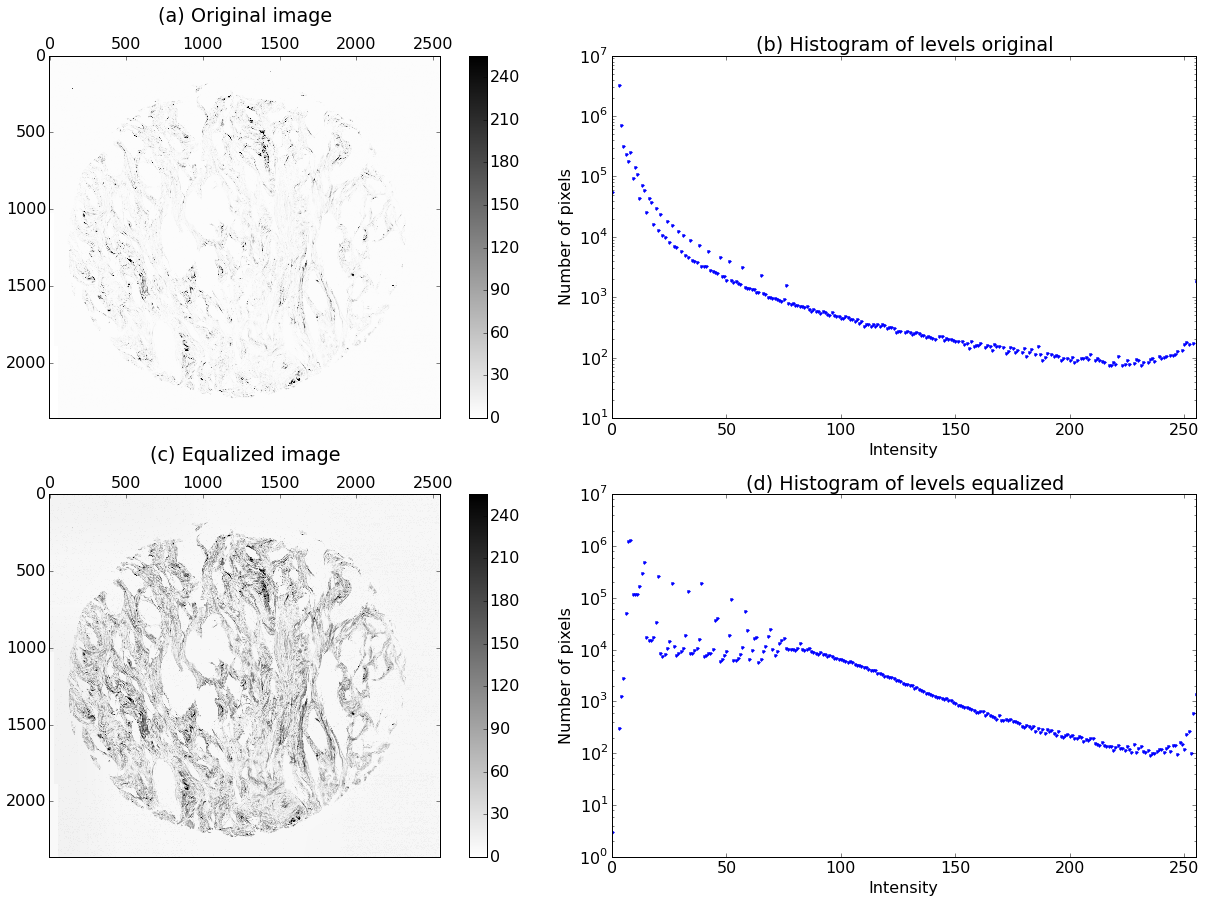
\includegraphics[width=14cm]{equalized}
\caption{(a) Original image from microscope. (b) Histrogram of intensity values in image (a). (c) Adaptive histogram equalization of image (a). (d) Histogram of intensity values in image (c). Note that the scale of the y-axis in the histograms are logarithmic. }
\label{fig:equalized}
\end{figure}

An image intensity value of zero equals no signal and representation is dependt on colormap chosen. As microscope images in this report tend to have a lot of near zero pixel values, an inverted colormap is used for better visibility. In other words zero are represented as white, in contrast to black that one might assume. As long as possible, the same colormap is used on same type of images. It is suggested that the reader note the colorbar beside the image which indicate correspondence between numerical value and color.

\subsection{Contrast enhancement}
Images where structures are more important than the numerical values, \textit{histogram equalization} is used to enhance contrast. Histogram equalization tries to make each intesity likely probable, which often result to a higher contrast and therefor better visibility. An example is shown in figure \ref{fig:equalized}, where (a) is the original image and (c) is the equalized image. The algorithm used to equalize figure \ref{fig:equalized} (c) is called \textit{adaptive histogram equalization} and are found in the python library scikit-image. As this are just for visibility in the report, it’s suggested to read scikit-image documentation or source code if more detail is needed. Figure caption will always note if images has been processed with any kind of contrast enhancement method.

%
% SCANNING MICROSCOPE
%
\section{Scanning microscope}
The microscope in use is a scanning microscope. It’s called scanning due to the moving mirror which directs the laser to different spatial coordinates on the sample. The laser will move in a raster pattern and a sensor detect light in samples. Each sample represent one pixel and computer software assign the sensed values to a digital image. By scanning speed, we mean the count of lines scanned per second. In example a scanning speed of 600 Hz will use 853 milliseconds to scan a whole image of 512x512 pixels.

As it’s possible to control the amplitude of the mirror oscillation, choosing a smaller amplitude of the oscillation will effectively zoom. This gives the user of a scanning microscope control over spatial resolution without changing objective. Though the zooming is not without limitation, as too high oscillation frequency could damage the mirror. In example, a high mirror oscillation frequency would limit the possible amplitude which effectively limits how low zoom one can use.

Even if it's possible in software to select resolution below the theoretical resolution defined by the Rayleigh criterion, we are still limited by the diffraction limit. Resolution is therefor given by

\begin{equation}
d = 0.61 \cdot \frac{\lambda}{NA}
\end{equation}

where $\lambda$ is wavelenght of light and $NA$ is numerical aperture of objective.

%
% NONLINEAR LIGHT INTERACTION
%
\section{Nonlinear light interaction}
%Signal, noise, sampling, instrumentation
Second harmonic generation (SHG) is a interaction between photons and material which generate light of twice the frequency as the incomming light. The generation is due to the material's nonlinear susceptibility, which can be explained by the polarized density

\begin{equation}
\vec{P} = \chi_1 \vec{E} + \chi_2 \vec{E} \cdot \vec{E} + \chi_3\vec{E} \cdot \vec{E} \cdot \vec{E} + ...
\end{equation}

When a material have $\chi_2 \neq 0$, two photons may interact with the material to create a polarized field. The polarized field then again generates an $\vec{E}$-field with twice the frequency as the incoming light (two photons interact with the material, creating a single photon with twice the energy). The interaction only happens upon a high intensity beam where two photons are at the same place at the same time. Practically this is achieved by using a pulsed laser and focusing the beam with an objective, as a steady beam of this intensity magnitude would damage the sample. Also since the probability for interaction is proportional to intensity squared, one get the convenient benefit of essentially no SHG outside the focal point.

$\chi_2$ is also dependent on wavelength of incoming light and properties of the material, which results in material needs to be non-centrocymetric. This happens to be the case for collagen fibers as some of few biological materials, making it simple to take images of the collagen fibers only with little sample preparation.

The pulsed laser is normally scanned over the sample, generating SHG-signal and detected by sensors. As compared to a confocal microscope, descanning of the light is not necessary to take away background signal. 

%
% FOURIER TRANSFORM
%
\section{Forier transform}
A common way to view data is in it's frequency domain. To achieve this, one does a Fourier transform defined by

\begin{equation}
F\{f(t)\} = \int \limits_{-\infty}^{\infty} f(t) e^{-i2\pi \mu t} dt.
\end{equation}

The transform has the property that it "picks out" amplitude and phase of oscillating signals in $f(t)$. This is based on the Fourier series which states that any periodic function can be represented by a sum of finite or infinite set of sines and cosines.

As we are working with images in the discrete domain, one defines $f(t)$ to be a sampled function using the Dirac delta function and gets the discrete Fourier transform

\begin{equation}
F(u) = \sum \limits_{x=0}^{M-1} f(x)e^{-i2 \pi ux/M}.
\end{equation}

Where $u$ and $x$ are discrete values for frequency and position, and M is number of samples in the function $f(x)$. Adding a dimension yields the 2D discrete Fourier transform given by

\begin{equation}
F(u,v) = \sum \limits_{x=0}^{M-1} \sum \limits_{y=0}^{N-1} f(x,y) e^{-i2 \pi \left( \frac{ux}{M} + \frac{vy}{N} \right)}.
\end{equation}

Here $u$ and $v$ are frequencies for accordingly $x$ and $y$ dimensions in the real image $f(x,y)$. $M$ and $N$ are the size of the image. The transform yields an image with same dimensions as the real image, where $F(u,v)$ gives amplitude and phase of given frequencies $u$ and $v$. All Fourier images in this report are logarithms of power spectrum which are shifted. The power spectrum of the Fourier transform is given by

\begin{equation}
|F(u,v)| = \sqrt{F(u,v) \cdot \overline{F(u,v)}},
\end{equation}

where $\overline{F(u,v)}$ is the complex conjugate of $F(u,v)$. Values below 1 are set to 1, to avoid division by zero and $-\infty$ values. Because the domain of values may range $10^6$ in the power spectrum, logarithmic scaling is done. In example the Fourier spectrum to figure \ref{fig:ft_demo} (a), have a maximum value of $8 \cdot 10^6$. Shifting means that $u=0$ and $v=0$ are set to the center of the image, as it's easier to grasp what frequencies are involved and direction of features in the image.

\begin{figure}[h]
\centering
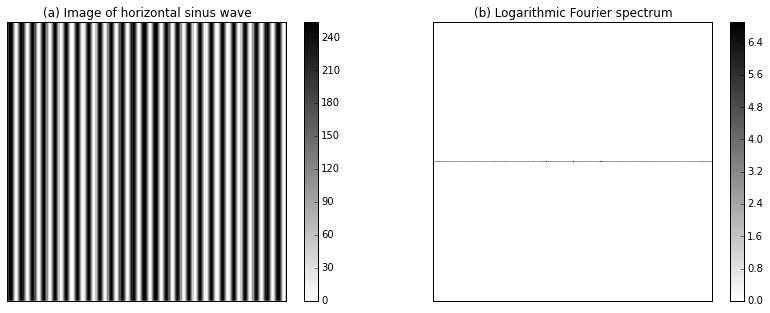
\includegraphics[width=11cm]{ft_demo.png}
\caption{(a) An 8 bit grayscale image with sine wave running in x-direction. (b) The logmarithmic scaled power spectrum of the Fourier transform. The Fourier transform has been shifted for better visibility, as we have no repeating signal in y-direction and the line actually lays on the border of the image ($v$ = 0).}
\label{fig:ft_demo}
\end{figure}

As mentioned, the transform picks out amplitude, phase and frequency, which are properties we can exploit to find orientation of fibers. Figure \ref{fig:ft_demo} shows this concept.


%
% CLASSIFICATION
%
%\section{Classification}
%Magnus: Mulig jeg må droppe dette, ser ikke ut som jeg kommer i mål.

%As the goal for automated analysis is making decisions, quantitative data is used to separate samples into classes. In best case scenario a few quantitative measurement clearly discriminates the samples. Figure \ref{fig:iris} of the classical iris data-set from R.A. Fisher illustrates this concept.

%\begin{figure}
%\centering
%\includegraphics[width=5cm]{iris.png}
%\caption{Three different species of iris flowers, discriminated by their pedal and sepal width. Data from http://archive.ics.uci.edu/ml/datasets/Iris. TODO fix ref}
%\label{fig:iris}
%\end{figure}

%As the figure show, grouping classes based on their quantitative measurements is a simple concept, but it gets complicated when the data span more dimensions that the human mind can easily visualize. To improve our ability to find good classifiers one technique is to use machine learning. The concept is the same, but one lets a computer find which measurements gives good separation of classes. This is done by iteratively computing distance to the mean position of predefined classes. Mean distance is defined as

%\begin{equation}
%\mathbf m_j = \frac{1}{N_j} \sum\limits_{\mathbf x \in \omega_j} \mathbf x_j
%\end{equation}

%where $N_j$ is the number of vectors in class $\omega_j$.


%A simple but effective implementation of this is clustering measurements 
%find quantitative measures that disciminates the samples to classes